% What one draw does: random_state_id() names the random state's handle,
% desc_use_side_effect() looks up (or, on the first use, creates) the trace's
% view of it, and passes the view's current value -- the key and the counter
% plus the draws before -- as the call's operands, counting the draw. How a view
% is created depends on the trace's side_effects_mode.
% Build: see figures/README.md
\documentclass[tikz, border = 6pt]{standalone}
\usepackage[T1]{fontenc}
\usepackage{lmodern}
\usepackage{amsmath}
\usetikzlibrary{positioning, calc, arrows.meta, fit, backgrounds}

\definecolor{hash}{HTML}{5B8C5A}
\definecolor{keep}{HTML}{2A7AB0}
\definecolor{fork}{HTML}{E08A2C}

\tikzset{
  >={Stealth[length = 2mm]},
  stage/.style = {draw = black!55, fill = white, rounded corners = 2pt,
    inner sep = 4pt, font = \footnotesize, align = left, text width = 6.3cm},
  code/.style = {font = \ttfamily\footnotesize},
  entry/.style = {draw = hash!80!black, fill = hash!12, rounded corners = 2pt,
    inner sep = 4pt, font = \footnotesize, align = left},
  mode/.style = {draw = keep!70!black, fill = keep!10, rounded corners = 2pt,
    inner sep = 3pt, font = \footnotesize, align = left, text width = 5.3cm},
  edge/.style = {->, black!60},
  lab/.style = {font = \footnotesize, text = black!60, fill = white, inner sep = 1pt}
}

\begin{document}
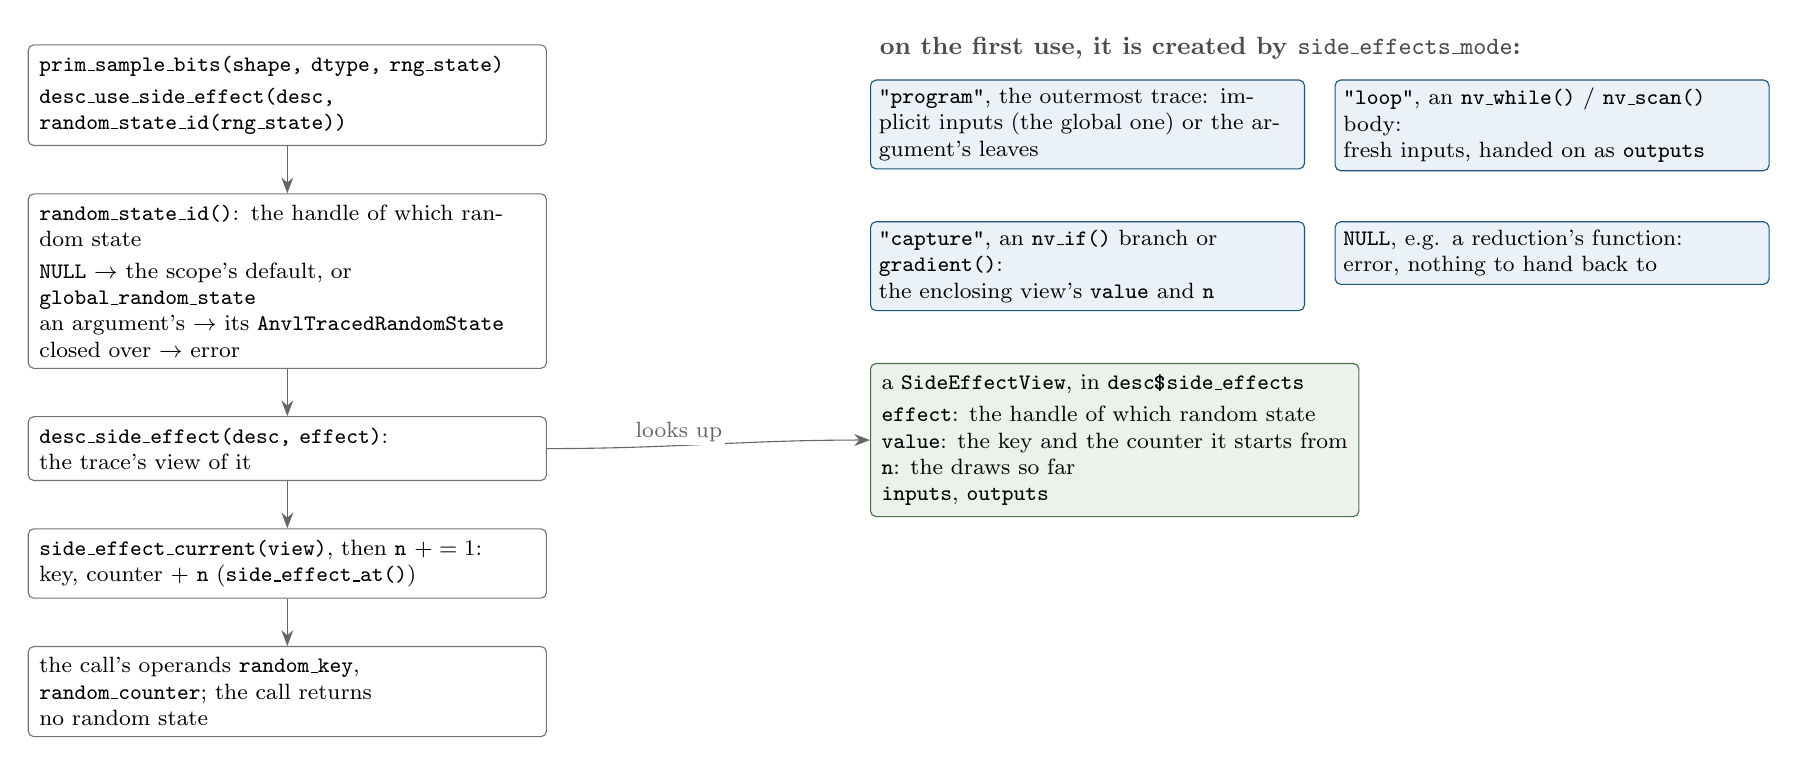
\begin{tikzpicture}

  \node[stage] (call) at (0, 0)
    {\texttt{prim\_sample\_bits(shape, dtype, rng\_state)}\\[2pt]
     \texttt{desc\_use\_side\_effect(desc, random\_state\_id(rng\_state))}};

  \node[stage, below = 0.6 of call] (id)
    {\texttt{random\_state\_id()}: the handle of which random state\\[2pt]
     \texttt{NULL} $\to$ the scope's default, or \texttt{global\_random\_state}\\
     an argument's $\to$ its \texttt{AnvlTracedRandomState}\\
     closed over $\to$ error};

  \node[stage, below = 0.6 of id] (view)
    {\texttt{desc\_side\_effect(desc, effect)}:\\
     the trace's view of it};

  \node[stage, below = 0.6 of view] (draw)
    {\texttt{side\_effect\_current(view)}, then \texttt{n} $+= 1$:\\
     key, counter $+$ \texttt{n} (\texttt{side\_effect\_at()})};

  \node[stage, below = 0.6 of draw] (ops)
    {the call's operands \texttt{random\_key},\\
     \texttt{random\_counter}; the call returns\\
     no random state};

  \foreach \a/\b in {call/id, id/view, view/draw, draw/ops} \draw[edge] (\a) -- (\b);

  % ---- the view ----------------------------------------------------------------
  \node[entry, anchor = north west] (entry) at (7.4, -3.4)
    {a \texttt{SideEffectView}, in \texttt{desc\$side\_effects}\\[2pt]
     \texttt{effect}: the handle of which random state\\
     \texttt{value}: the key and the counter it starts from\\
     \texttt{n}: the draws so far\\
     \texttt{inputs}, \texttt{outputs}};
  \draw[edge] (view.east) to[out = 0, in = 180] node[lab, above, pos = 0.4] {looks up} (entry.west);

  % ---- first use: by mode -------------------------------------------------------
  \node[font = \small\bfseries, text = black!70, anchor = west] at (7.4, 0.6)
    {on the first use, it is created by \texttt{side\_effects\_mode}:};
  \node[mode, anchor = north west] (m1) at (7.4, 0.2)
    {\texttt{"program"}, the outermost trace: implicit inputs (the global one) or
     the argument's leaves};
  \node[mode, anchor = north west] (m2) at (13.3, 0.2)
    {\texttt{"loop"}, an \texttt{nv\_while()} / \texttt{nv\_scan()} body:\\
     fresh inputs, handed on as \texttt{outputs}};
  \node[mode, anchor = north west] (m3) at (7.4, -1.6)
    {\texttt{"capture"}, an \texttt{nv\_if()} branch or \texttt{gradient()}:\\
     the enclosing view's \texttt{value} and \texttt{n}};
  \node[mode, anchor = north west] (m4) at (13.3, -1.6)
    {\texttt{NULL}, e.g. a reduction's function:\\error, nothing to hand back to};

\end{tikzpicture}
\end{document}
